\section{二阶条件}
\label{sec:kkt-second-order}

KKT点可能是最小点，也可能不是。单位圆周上最小化$\frac12\lVert\bm{x}-(2,0)\rVert_2^2$就是例子：离$(2,0)$最近和最远的点都满足一阶条件。这就需要回答：一阶信息判断不了的时候，曲率怎样作出判断？这需要先确定该检查哪些方向，再确定该检查谁的曲率。

\subsection{临界锥}
\label{sec:kkt-critical-cone}

设$(\bm{x}^\star,\bm{\lambda}^\star,\bm{\nu}^\star)$是KKT点。对线性化方向$\bm{d}\in\bm{F}(\bm{x}^\star)$，由驻定条件，目标的一阶变化是
\[
 \langle\nabla f(\bm{x}^\star),\bm{d}\rangle=-\sum_{i\in A(\bm{x}^\star)}\lambda_i^\star\langle\nabla g_i(\bm{x}^\star),\bm{d}\rangle-\sum_{j=1}^p\nu_j^\star\langle\nabla h_j(\bm{x}^\star),\bm{d}\rangle.
\]
等式项为零。每个$\lambda_i^\star\geq0$，每个$\langle\nabla g_i,\bm{d}\rangle\leq0$，所以右端是非负项之和。

若这个值严格为正，目标沿$\bm{d}$一阶上升，这个方向已经判决完毕，二阶项不用看。需要继续检查的，只有一阶变化恰好为零的方向。一个非负项之和为零，当且仅当每一项为零，所以这些方向在$\lambda_i^\star>0$的活动约束上必须取等号。

\begin{definition}[临界锥]
\label{def:kkt-critical-cone}
设$(\bm{x}^\star,\bm{\lambda}^\star,\bm{\nu}^\star)$是KKT点。集合
\begin{equation}
 \bm{K}(\bm{x}^\star,\bm{\lambda}^\star)=\left\{\bm{d}\in\bm{F}(\bm{x}^\star):
 \langle\nabla g_i(\bm{x}^\star),\bm{d}\rangle=0\ \text{对所有}\ \lambda_i^\star>0
 \right\}
 \label{eq:kkt-critical-cone}
\end{equation}
称为\term{临界锥}（critical cone）。由上面的推导，它等于
\begin{equation}
 \bm{K}(\bm{x}^\star,\bm{\lambda}^\star)=\{\bm{d}\in\bm{F}(\bm{x}^\star):\langle\nabla f(\bm{x}^\star),\bm{d}\rangle=0\}.
 \label{eq:kkt-critical-cone-f}
\end{equation}
\end{definition}

式~\eqref{eq:kkt-critical-cone-f}的右端不含乘子，所以即使乘子不唯一，临界锥也不依赖乘子的选择。两种写法各有用处：式~\eqref{eq:kkt-critical-cone}便于计算，式~\eqref{eq:kkt-critical-cone-f}说明它的含义。

零乘子的活动约束值得单独看。这样的约束在式~\eqref{eq:kkt-critical-cone}里没有被要求取等号，它仍然保留$\langle\nabla g_i,\bm{d}\rangle\leq0$的单侧限制。所以临界锥一般是锥，不是子空间。

用预算例算三种情况，见图~\ref{fig:kkt-critical-cone}。$\tau=1/2$的角点，$\lambda_1,\lambda_3$都为正，两条约束都取等号，$d_1+d_2=0$，$d_2=0$，于是$\bm{K}=\{\bm{0}\}$：一阶条件已经判决了所有方向。

$\tau=1$的角点$(1,0)$，$\lambda_1=1>0$，$\lambda_3=0$，于是$g_1$取等号，$g_3$只保留单侧：
\[
 \bm{K}=\{\bm{d}:d_1+d_2=0,\ d_2\geq0\}=\{s(-1,1):s\geq0\}.
\]
沿预算线向上走的这一条射线，一阶变化为零，要靠二阶项判断。而反方向$(1,-1)$不可行。

\begin{BookInlineFigure}
  \centering
  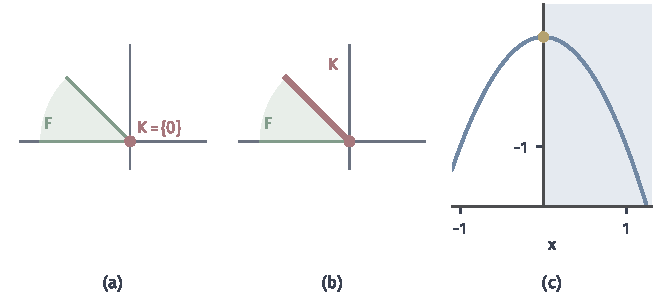
\includegraphics[width=112mm]{figures/05-optimization/06-constrained-optimization/matplotlib/kkt-critical-cone/figure.pdf}
  \caption{临界锥（红色）与线性化锥$\bm{F}$（绿色）。(a)预算例$\tau=1/2$的角点，两个乘子都为正，$\bm{K}=\{\bm{0}\}$。(b)预算例$\tau=1$的角点，$\lambda_3=0$，$\bm{K}$是射线$s(-1,1)$，$s\geq0$。(c)$\min-x^2$，$x\geq0$（蓝色带），黄点$x=0$是KKT点，乘子为零，$\bm{K}=[0,\infty)$。}
  \label{fig:kkt-critical-cone}
\end{BookInlineFigure}

\paragraph{不能把活动约束都当成等式}
一种常见的简化是把所有活动约束当成等式，对每个活动的$g_i$都要求$\langle\nabla g_i,\bm{d}\rangle=0$。下面的例子说明这样会漏掉下降方向。最小化$f(x)=-x^2$，约束$g(x)=-x\leq0$。在$x=0$处，$f'(0)=0$，所以$\lambda=0$，KKT条件成立。

约束活动而乘子为零，真正的临界锥是$\{d:-d\leq0\}=[0,\infty)$。沿$d=1$，$f''(0)d^2=-2<0$，二阶检验发现$x=0$不是局部最小点，事实上$f(t)=-t^2<0$。

要是把约束当成等式，方向只剩$\{0\}$，就没有方向可供检查，会错误地接受$x=0$。图~\ref{fig:kkt-critical-cone}(c)就是这个例子。

\subsection{二阶必要条件}
\label{sec:kkt-sonc}

下一个问题是该检查谁的曲率。答案不是目标的Hessian，用下面的例子就能看清。

\paragraph{约束的弯曲进入曲率}
在单位圆周上最小化$f(\bm{x})=\frac12[(x_1-2)^2+x_2^2]$，也就是找圆周上离$(2,0)$最近的点。令$h(\bm{x})=x_1^2+x_2^2-1$，驻定条件是
\[
 x_1-2+2\nu x_1=0,\qquad x_2+2\nu x_2=0.
\]
第二式说明$x_2=0$或$\nu=-1/2$。后者代入第一式得$-2=0$，不可能，所以$x_2=0$，$x_1=\pm1$。两个KKT点是
\[
 (1,0),\ \nu=\frac12;\qquad(-1,0),\ \nu=-\frac32.
\]

这两点的目标Hessian都是单位阵，正定，分不开。用角度参数化圆周，目标变成
\[
 \phi(\theta)=f(\cos\theta,\sin\theta)=\frac52-2\cos\theta,\qquad\phi''(\theta)=2\cos\theta.
\]
在$(1,0)$处$\phi''=2$，是极小；在$(-1,0)$处$\phi''=-2$，是极大。图~\ref{fig:kkt-constraint-curvature}(b)的黄色抛物线就是这两个曲率。

\begin{BookInlineFigure}
  \centering
  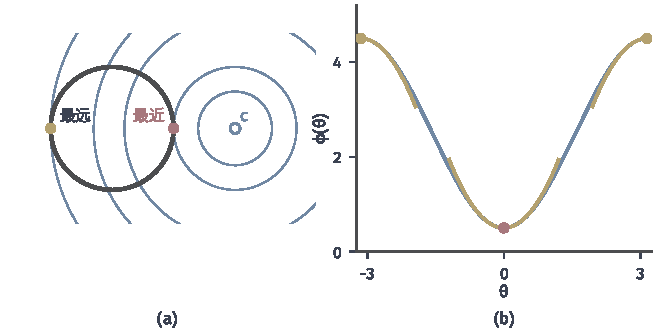
\includegraphics[width=112mm]{figures/05-optimization/06-constrained-optimization/matplotlib/kkt-constraint-curvature/figure.pdf}
  \caption{约束的弯曲改变了有效曲率。(a)深灰圆是可行集，蓝线是目标$\frac12\lVert\bm{x}-\bm{c}\rVert_2^2$（$\bm{c}=(2,0)$）的等高线。红点$(1,0)$是最近点，黄点$(-1,0)$是最远点，两者都是KKT点，目标Hessian都是单位阵。(b)沿圆周的目标值$\phi(\theta)=5/2-2\cos\theta$，黄色抛物线是两点处曲率分别为$2$、$-2$的二次近似。}
  \label{fig:kkt-constraint-curvature}
\end{BookInlineFigure}

这两个数从哪里来？沿可行曲线$\bm{x}(t)$，$\bm{x}(0)=\bm{x}^\star$，$\bm{x}'(0)=\bm{d}$，复合函数求二阶导数得到
\[
 \frac{\mathrm{d}^2}{\mathrm{d}t^2}f(\bm{x}(t))\Big|_{t=0}=\bm{d}^\top\nabla^2f(\bm{x}^\star)\bm{d}+\langle\nabla f(\bm{x}^\star),\bm{x}''(0)\rangle.
\]
第二项是曲线的弯曲$\bm{x}''(0)$贡献的，它是约束带来的，只看目标Hessian看不到这一项。

对恒等式$h(\bm{x}(t))=0$同样求两次导数，得到
\[
 \bm{d}^\top\nabla^2h(\bm{x}^\star)\bm{d}+\langle\nabla h(\bm{x}^\star),\bm{x}''(0)\rangle=0.
\]
再由驻定条件$\nabla f=-\nu\nabla h$，弯曲项可以用约束的Hessian表示：
\[
 \langle\nabla f(\bm{x}^\star),\bm{x}''(0)\rangle=-\nu\langle\nabla h(\bm{x}^\star),\bm{x}''(0)\rangle=\nu\,\bm{d}^\top\nabla^2h(\bm{x}^\star)\bm{d}.
\]

两式合起来，沿曲线的二阶导数恰好是
\[
 \bm{d}^\top\bigl(\nabla^2f(\bm{x}^\star)+\nu\nabla^2h(\bm{x}^\star)\bigr)\bm{d},
\]
括号里是Lagrange函数对$\bm{x}$的Hessian。乘子把约束的弯曲折算成了目标的曲率。在例子中$\nabla^2h=2\bm{I}$，$\bm{d}=(0,1)$，代入$(1,0)$得$1+2\cdot\frac12=2$，代入$(-1,0)$得$1+2\cdot(-\frac32)=-2$，与$\phi''$完全一致。

一般地，把Lagrange函数对$\bm{x}$的Hessian记为
\begin{equation}
 \nabla^2_{\bm{x}\bm{x}}\mathcal{L}(\bm{x},\bm{\lambda},\bm{\nu})=\nabla^2f(\bm{x})+\sum_{i=1}^m\lambda_i\nabla^2g_i(\bm{x})+\sum_{j=1}^p\nu_j\nabla^2h_j(\bm{x}).
 \label{eq:kkt-lagrangian-hessian}
\end{equation}

\begin{theorem}[二阶必要条件]
\label{thm:kkt-sonc}
设$f$、$g_i$、$h_j$在局部最小点$\bm{x}^\star$附近二阶连续可微，$\bm{x}^\star$满足LICQ，$(\bm{\lambda}^\star,\bm{\nu}^\star)$是它唯一的KKT乘子。则
\begin{equation}
 \bm{d}^\top\nabla^2_{\bm{x}\bm{x}}\mathcal{L}(\bm{x}^\star,\bm{\lambda}^\star,\bm{\nu}^\star)\bm{d}\geq0
 \quad\text{对所有}\ \bm{d}\in\bm{K}(\bm{x}^\star,\bm{\lambda}^\star).
 \label{eq:kkt-sonc}
\end{equation}
\end{theorem}

\begin{proof}
取$\bm{d}\in\bm{K}$，令
\[
 W=\{i\in A(\bm{x}^\star):\langle\nabla g_i(\bm{x}^\star),\bm{d}\rangle=0\}.
\]
由临界锥的定义，$\lambda_i^\star>0$的下标都在$W$中。LICQ保证引理~\ref{lem:kkt-feasible-curve}适用，得到二阶连续可微的可行曲线$\bm{x}(t)$，$0\leq t<\delta$，它沿$\bm{d}$出发，并使$h_j$与$g_i$（$i\in W$）恒为零。

令$\phi(t)$是乘子固定为$(\bm{\lambda}^\star,\bm{\nu}^\star)$时Lagrange函数沿曲线的值。曲线上等式约束为零，$i\in W$的约束为零，其余约束的乘子为零，所以对$0\leq t<\delta$，
\[
 \phi(t)=\mathcal{L}(\bm{x}(t),\bm{\lambda}^\star,\bm{\nu}^\star)=f(\bm{x}(t)).
\]
这是使用Lagrange函数的好处：在这条曲线上，它和目标完全一样，但它的梯度在$\bm{x}^\star$处为零。

由驻定条件，
\[
 \phi'(0)=\langle\nabla_{\bm{x}}\mathcal{L}(\bm{x}^\star,\bm{\lambda}^\star,\bm{\nu}^\star),\bm{d}\rangle=0.
\]
再求一次导数，含$\bm{x}''(0)$的项同样因$\nabla_{\bm{x}}\mathcal{L}=\bm{0}$消失，得到
\[
 \phi''(0)=\bm{d}^\top\nabla^2_{\bm{x}\bm{x}}\mathcal{L}(\bm{x}^\star,\bm{\lambda}^\star,\bm{\nu}^\star)\bm{d}.
\]

$\bm{x}(t)$可行且趋于局部最小点，所以小的$t>0$时$\phi(t)\geq\phi(0)$。由Taylor公式，$\phi(t)-\phi(0)=\frac12\phi''(0)t^2+o(t^2)$，除以$t^2$并令$t\downarrow0$，得到$\phi''(0)\geq0$。
\end{proof}

定理中的LICQ负责把每个临界方向实现成可行曲线。没有约束资格时，临界方向可能只是线性化的产物。最小化$-x^2$，约束$x^2\leq0$，原点是唯一可行点，取乘子$\lambda=0$是一组KKT乘子，此时$\nabla^2_{xx}\mathcal{L}=-2$，$\bm{K}=\mathbb{R}$，式~\eqref{eq:kkt-sonc}不成立，而原点当然是最小点。

\paragraph{两种错误的简化}
条件~\eqref{eq:kkt-sonc}既不等同于目标Hessian半正定，也不等同于在全空间半正定。圆周例已经说明目标Hessian可以正定而点不是局部最小点。

反过来，全空间的不定性也不妨碍极小。最小化$x_1^2-x_2^2$，约束$x_2=0$，原点处$\nu=0$，Lagrange Hessian是$\operatorname{diag}(2,-2)$，不定。但临界锥是$\{\bm{d}:d_2=0\}$，上面的二次型是$2d_1^2\geq0$。原点确实是最小点，负曲率的方向被约束禁止了。

\subsection{二阶充分条件}
\label{sec:kkt-sosc}

必要条件是用来排除的，充分条件是用来确认的。把不等号换成严格，就能确认局部最优，并且还能给出增长的速度。值得注意的是，这里不需要约束资格。

\begin{theorem}[二阶充分条件]
\label{thm:kkt-sosc}
设$f$、$g_i$、$h_j$在$\bm{x}^\star$附近二阶连续可微，$(\bm{x}^\star,\bm{\lambda}^\star,\bm{\nu}^\star)$是KKT点，并且
\begin{equation}
 \bm{d}^\top\nabla^2_{\bm{x}\bm{x}}\mathcal{L}(\bm{x}^\star,\bm{\lambda}^\star,\bm{\nu}^\star)\bm{d}>0
 \quad\text{对所有非零}\ \bm{d}\in\bm{K}(\bm{x}^\star,\bm{\lambda}^\star).
 \label{eq:kkt-sosc}
\end{equation}
则存在$\sigma>0$，$r>0$，使
\begin{equation}
 f(\bm{x})\geq f(\bm{x}^\star)+\sigma\lVert\bm{x}-\bm{x}^\star\rVert_2^2
 \quad\text{对所有}\ \bm{x}\in\bm{C},\ \lVert\bm{x}-\bm{x}^\star\rVert_2<r.
 \label{eq:kkt-quadratic-growth}
\end{equation}
特别地，$\bm{x}^\star$是严格局部最小点。
\end{theorem}

\begin{proof}
反设结论不成立。对每个$k$取$\sigma=1/k$，存在可行点$\bm{x}^{(k)}\neq\bm{x}^\star$，$\bm{x}^{(k)}\to\bm{x}^\star$，使
\[
 f(\bm{x}^{(k)})<f(\bm{x}^\star)+\frac1k\lVert\bm{x}^{(k)}-\bm{x}^\star\rVert_2^2.
\]
记$t_k=\lVert\bm{x}^{(k)}-\bm{x}^\star\rVert_2$，$\bm{d}^{(k)}=(\bm{x}^{(k)}-\bm{x}^\star)/t_k$。单位向量列有收敛子列，不妨设$\bm{d}^{(k)}\to\bm{d}$，$\lVert\bm{d}\rVert_2=1$。按定义~\ref{def:kkt-tangent-cone}，$\bm{d}$是切向量，由定理~\ref{thm:kkt-tangent-in-linearized}，$\bm{d}\in\bm{F}(\bm{x}^\star)$。

\emph{第一步：$\bm{d}$是临界方向。}上面的不等式减去$f(\bm{x}^\star)$，除以$t_k$，令$k\to\infty$，得到$\langle\nabla f(\bm{x}^\star),\bm{d}\rangle\leq0$。第~\ref{sec:kkt-critical-cone}节已经证明，$\bm{d}\in\bm{F}$时这个内积是非负项之和，所以它等于零。由式~\eqref{eq:kkt-critical-cone-f}，$\bm{d}\in\bm{K}$。

\emph{第二步：比较Lagrange函数。}下面乘子固定为$(\bm{\lambda}^\star,\bm{\nu}^\star)$，把Lagrange函数简记为$\mathcal{L}(\bm{x})$。$\bm{x}^{(k)}$可行，$\bm{\lambda}^\star\geq\bm{0}$，所以$\mathcal{L}(\bm{x}^{(k)})\leq f(\bm{x}^{(k)})$。由互补松弛和等式约束，$\mathcal{L}(\bm{x}^\star)=f(\bm{x}^\star)$。于是
\[
 \mathcal{L}(\bm{x}^{(k)})-\mathcal{L}(\bm{x}^\star)\leq f(\bm{x}^{(k)})-f(\bm{x}^\star)<\frac{t_k^2}{k}.
\]

\emph{第三步：展开。}在$\bm{x}^\star$处$\nabla_{\bm{x}}\mathcal{L}=\bm{0}$，由二阶Taylor公式，
\[
 \mathcal{L}(\bm{x}^{(k)})-\mathcal{L}(\bm{x}^\star)=\frac{t_k^2}{2}(\bm{d}^{(k)})^\top\nabla^2_{\bm{x}\bm{x}}\mathcal{L}(\bm{x}^\star)\bm{d}^{(k)}+o(t_k^2).
\]
代入上式，除以$t_k^2$，令$k\to\infty$，得到
\[
 \frac12\bm{d}^\top\nabla^2_{\bm{x}\bm{x}}\mathcal{L}(\bm{x}^\star)\bm{d}\leq0.
\]
这与式~\eqref{eq:kkt-sosc}矛盾。
\end{proof}

证明从头到尾没有用到切锥等于线性化锥，只用了$\bm{T}_{\bm{C}}\subseteq\bm{F}$这个总成立的方向，所以不需要约束资格。它也只要求某一组KKT乘子满足式~\eqref{eq:kkt-sosc}。

在圆周的最近点$(1,0)$，$\bm{K}=\{(0,s)\}$，$\nabla^2_{\bm{x}\bm{x}}\mathcal{L}=2\bm{I}$，条件成立。这里增长式可以精确写出。圆周上，
\[
 f(\bm{x})-\frac12=2-2\cos\theta=\lVert\bm{x}-(1,0)\rVert_2^2,
\]
所以$\sigma=1$。

临界锥只有零向量时，条件~\eqref{eq:kkt-sosc}自动成立，这时一阶条件就足以确认严格局部最小。预算例$\tau=1/2$的角点就是这样。

\paragraph{条件的边界}
严格正性不能放松成半正定。图~\ref{fig:kkt-degenerate-curvature}中三个一元函数在原点的二阶导数都是零，临界锥都是全空间，半正定都成立，可是$x^3$和$-x^4$的原点都不是局部最小点。

严格正性也不是必要的。$x^4$的原点是严格局部最小点，二阶导数却是零。所以二阶必要条件和二阶充分条件之间有一条缝，缝里的情形要靠更高阶的信息或问题的特殊结构。

\begin{BookInlineFigure}
  \centering
  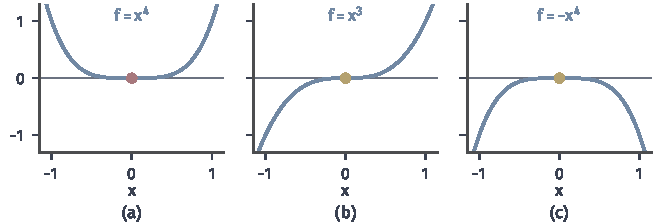
\includegraphics[width=112mm]{figures/05-optimization/06-constrained-optimization/matplotlib/kkt-degenerate-curvature/figure.pdf}
  \caption{二阶导数为零时，二阶条件无法判决。(a)$x^4$：原点（红）是严格局部最小点。(b)$x^3$：原点（黄）不是局部极值点。(c)$-x^4$：原点（黄）是最大点。三者在原点的一、二阶导数都是零。}
  \label{fig:kkt-degenerate-curvature}
\end{BookInlineFigure}

表~\ref{tab:kkt-second-order}对比这两个条件。

\begin{BookInlineTable}
  \centering
  \begin{tabular}{@{}lll@{}}
    \toprule
    对比项 & 二阶必要条件 & 二阶充分条件\\
    \midrule
    出发点 & 已知局部最小点 & 已知KKT点\\
    约束资格 & 需要LICQ & 不需要\\
    二次型 & 在$\bm{K}$上$\geq0$ & 在$\bm{K}$的非零向量上$>0$\\
    结论 & 用于排除候选点 & 严格局部最小，二次增长\\
    \bottomrule
  \end{tabular}
  \caption{二阶必要条件与二阶充分条件的比较。}
  \label{tab:kkt-second-order}
\end{BookInlineTable}

\paragraph{完整走一遍}
最后用一个非凸问题把各项检查串起来：
\begin{equation}
 \min_{\bm{x}\in\mathbb{R}^2}\ -x_1x_2\quad\text{s.t.}\quad g(\bm{x})=x_1^2+x_2^2-2\leq0.
 \label{eq:kkt-full-example}
\end{equation}
可行集是紧的圆盘，目标连续，最小点存在。圆盘内部没有活动约束，边界上$\nabla g=2\bm{x}\neq\bm{0}$，所以LICQ在每个可行点成立，每个局部最小点都满足KKT条件。

驻定条件是
\[
 -x_2+2\lambda x_1=0,\qquad-x_1+2\lambda x_2=0.
\]
由第一式得$x_2=2\lambda x_1$，代入第二式得$x_1=4\lambda^2x_1$。所以要么$x_1=0$，这时$x_2=0$；要么$4\lambda^2=1$。

若$x_1\neq0$，$\lambda=\pm1/2$，都不等于零，互补松弛要求约束活动。$\lambda=1/2$时$x_2=x_1$，代入$g=0$得到$(1,1)$与$(-1,-1)$。$\lambda=-1/2$时$x_2=-x_1$，得到$(1,-1)$与$(-1,1)$，但乘子为负，违反式~\eqref{eq:kkt-dual}，这两点被排除。负乘子说明从这两点沿半径向内走，目标反而下降，这两点其实是最大点。

留下三个KKT点，用二阶条件判决。在原点，$\lambda=0$，$\bm{K}=\mathbb{R}^2$，Hessian和$\bm{d}=(1,1)$给出
\[
 \nabla^2_{\bm{x}\bm{x}}\mathcal{L}=\begin{bmatrix}0&-1\\-1&0\end{bmatrix},\qquad\bm{d}^\top\nabla^2_{\bm{x}\bm{x}}\mathcal{L}\,\bm{d}=-2<0.
\]
原点不满足二阶必要条件，不是局部最小点。

在$(1,1)$，$\lambda=1/2>0$，临界锥要求$\langle\nabla g,\bm{d}\rangle=2d_1+2d_2=0$，即$\bm{d}=s(1,-1)$。Lagrange Hessian是
\[
 \nabla^2_{\bm{x}\bm{x}}\mathcal{L}=\begin{bmatrix}1&-1\\-1&1\end{bmatrix},\qquad\bm{d}^\top\nabla^2_{\bm{x}\bm{x}}\mathcal{L}\,\bm{d}=4s^2>0\ \ (s\neq0).
\]
这个矩阵只是半正定，在$(1,1)$方向为零，但$(1,1)$不是临界方向。二阶充分条件成立，$(1,1)$是严格局部最小点。$(-1,-1)$由对称性相同。

全局最小点存在，又一定在KKT点中。比较目标值，$f(\pm(1,1))=-1$，$f(\bm{0})=0$，所以最优值是$-1$，全局最小点是这两点。这一步用的是“存在性、约束资格、枚举全部候选”这一套全局论证，单靠二阶条件得不到。图~\ref{fig:kkt-full-example}把五个候选点标在一起。

\begin{BookInlineFigure}
  \centering
  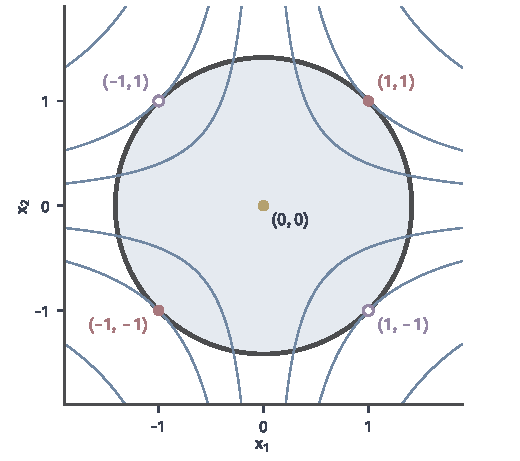
\includegraphics[width=88mm]{figures/05-optimization/06-constrained-optimization/matplotlib/kkt-full-example/figure.pdf}
  \caption{问题~\eqref{eq:kkt-full-example}的候选点。浅蓝圆盘是可行集，蓝线是$-x_1x_2$的等高线。红点$\pm(1,1)$是全局最小点。黄点$(0,0)$是KKT点，但二阶必要条件不成立。紫色空心点$\pm(1,-1)$满足驻定和活动条件，乘子为$-1/2$，不是KKT点。}
  \label{fig:kkt-full-example}
\end{BookInlineFigure}
